\chapter{State of the art}
This chapter summarizes already existing technologies and implementations that are relevant to the library. Despite the fact that most of them are written in the C language, they are still relevant as they describe how many operating systems work and where many C++ standards come from.   
\section{Current Situation} 
At the time of writing this (December 2021), there are four mostly used architectures in the IT-Branch. These are Windows, Linux and MacOS. Linux was developed with the UNIX system as its core, while MacOS is only based on UNIX, which means that these are similar but not entirely compatible with each other. The big difference comes with Windows.\\
\footnotetext{Some companies also use ARM(aarch64), but this is not an OS and per default doesn't come with any process control system. In order to do so one needs to write or use an extra library for that solely purpose}Each operating system can deliver informations about its own computer.
For that, each of them has its own unique program. Windows uses the \dq Task-Manger\dq{} which comes with a GUI and shows real-time information about the CPU and memory of the computer, it comes with a list of processes and makes it possible for the user to manage them with only a couple of clicks.\\
Linux on the other hand is more text oriented. This operating system comes with a built in command called "top". This also delivers informations about your system, but it doesn't allow you to manipulate processes like \dq Task-manger\dq{} does. Although not very practicable for developers, these tools allow the user to measure performance in a normal state where your computer is not put under pressure, whereas the most interesting state is when the CPU needs to do a lot of operations and it needs to share its valuable time with other processes. To force such situations, the user can use online stress tests, which use the browser as an workload source, which for many is not very practicable, because it uses an additional program, that runs in the background. Online stress tests rely on internet to work and a stable ethernet or wifi connection to work. This way the results can be very inaccurate if the the network is under pressure.
\begin{figure}[h]
	\centering
	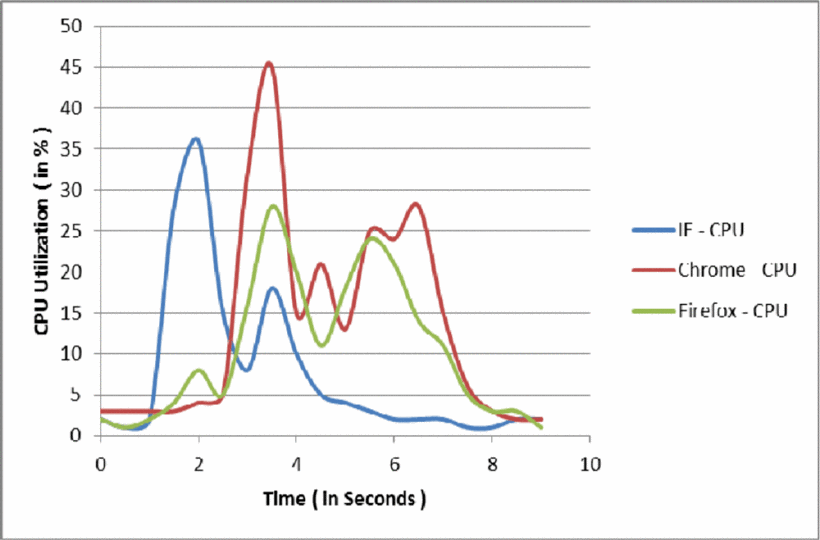
\includegraphics[scale=0.25]{figures/einleitung/browser_comparisson.png}
	\caption{Browser CPU utilization comparison\cite{6724273}}
	\label{browser_comp}
\end{figure}
\\
There are already some alternative libraries on the internet to recreate this method, but most of them are written in other programming languages. Adding them to a C++ Project would rise the complexity of the source code.\\
Some people would think "Well C++ is a new and modern language. There must be something similar out there". This statement is true and because of its young age there are a limited number of officially tested methods. You could also take a look at the headers implemented in the \href{https://en.cppreference.com/w/cpp/header}{C++ standard library} \cite{CppRef} to familiarize yourself with common algorithms and data structures.
Not all operating systems will be covered in this thesis.
The following statements are true for the testing machines used in chapter 4?.
\section{Processes}
To many operating systems, a process is like a wrapper defined by the kernel in order to allocate resources to an executing program.\\
When a process is created the system assigns him a \textit{process unique identifier} also called PID(a positive integer). Each process has its own PID, so two different executing programs cannot have the same PID \footnote{On UNIX like machines the first process to be called is the init process with PID 1}. The methods used to create a new process differ on each operating systems.
On Windows you can create processes by calling the \texttt{CreateProcessA()} function \cite{createProcWinAPI}, which returns a HANDLE (the equivalent PID for windows systems) and on linux you can use \texttt{fork()}\cite{LPI}. Each operating system calls one these methods internally every time the computer or the user starts a routine of execution, like starting a service, or a program (browser, spotify, etc). You can think of this system like a binary tree with one or more children with the kernel on top. The children have also an additional attribute called PPID, that contains the PID of its creator. If this is specified to zero then the kernel is the parent.\cite{wikiPPID}\footnote{There a very few processes that have the PPID=0 (ex. init)}.
\subsection{Threads} 
Each process has at least one thread of execution called the main thread, which (as the name says) contains the \texttt{main()} function, that defines the behavior of that process. The main thread can also create other threads that work independently from one another. On UNIX systems one would use the \texttt{pthread\_create()} and on windows \texttt{Create\_Thread()}. Once a thread has been created, the main thread can wait for it to finish by calling a method called \texttt{join()} and then resume execution or if the created thread called \texttt{detach()}, so it will separate itself from the main thread. This way the main thread doesn't have to wait for it to terminate and when a detached thread exists, all of his allocated resources will automatically be freed.\\
Like processes, threads also have unique identifiers called \textit{Thread identifiers} or TID and OS-specific methods to create them. But the role of this library is to make this whole process as transparent as possible, so we will use the C++ Standard Library's threads (std::thread) and \dq detach\dq{} ourselves from the other ones.\\
Processes have their own stack, so they can't communicate with each other. This is a huge problem when it comes concurrency (explained in \autoref{ssec:concurrency}), but threads share the stack of their creator-process.
\subsection{Differences between threads and processes} 
Many people tend to think of threads and processes as being the same, but they are quite different. First, as mentioned above, threads share the same stack of the creator-process, while processes need intercommunication tools like pipes to talk to each other. Another difference is that a process can have multiple threads attached to it, but a thread cannot belong to more than one process (but this doesn't stop a thread to call \texttt{fork()} and so create another process).\footnote{If the execution method of a thread calls \texttt{fork()} then that process's PPID will be the PID of thread's creator}. Their identifiers are also independent from their creator's. This way a TID can be equal to its creator's (or another process's) PID. For example if a process has its PID equal to 2033, there is no rule that will stop the thread having the same number as its TID. \\
To summarize and simplify the whole concept, one can imagine a process like an octopus and the threads being it's arms. One octopus has many arms that can execute multiple tasks at the same time, but an arm cannot belong to more than one octopus.\\
In this library we use multiple threads to simulate a user-specific workload\footnote{The user can set the wished workload with a simple function}, because this way we can time their execution start point with only one shared variable and we don't have to worry about interprocess communications. 
\subsection{Attributes}
Normally when we would create a threads using the unix methods, we would pass a pointer to a
structure that describes the attributes for that specific thread(that structure can be created with 
\texttt{pthread\_attr\_init()} and be destroyed with \texttt{pthread\_attr\_destroy()}). Some of these attributes include the 
scheduling priority, scheduling policy and stack size, which are important for out tests. 
Unfortunately the standard library doesn't have this option. In order to set and get this attributes
we need to use the architecture's dependent functions. In the following sections the attributes of a thread will be discussed.
\section{Stack Size}
\begin{wrapfigure}{1}{0.5\textwidth}
	\centering
	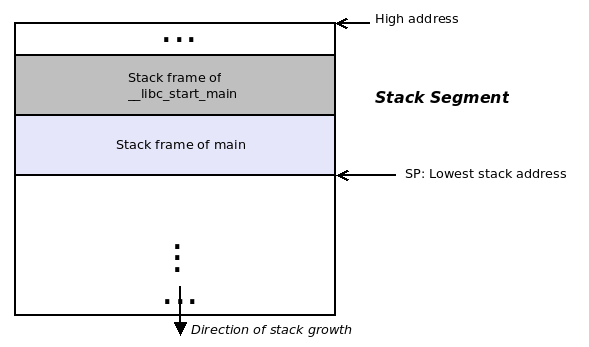
\includegraphics[width=.98\linewidth]{../figures/systemgrundlagen/stack.png}
	\caption{Stack segment}
	\cite{stack}
\end{wrapfigure}
The stack is a piece of memory where meta-data and local variables are saved when the \texttt{main()} function calls a routine/method. This memory segment is limited and doesn't allow an infinite number of data segments (also called stack frames) being stored in it. The stack uses assembly instruction like \texttt{pop} to delete a frame and \texttt{push} to add a frame. For consistency the stack will always pop the last element pushed. This is also known as \dq Last in First Out\dq{}\cite{stack}.\\
On UNIX systems we would create an attribute structure and pass the
desired options there. However, because we don't use the unix's system function \texttt{pthread\_create()} we also
cannot use the attribute structure. Furthermore the standard library doesn't support such tweaks. 
This is very important if someone wants to use this for an ARM architecture, because he won't be
able to define a meaningful stack size. This doesn't pose any threats for many operating systems out
there, but for ARM, which has a limited stack size, can be problematic. For windows this attribute
can be set using the \texttt{Create\_Thread()} function just like in unix using \texttt{pthread\_create()}.
\section{Concurrency}
\label{ssec:concurrency}
Concurrency means that two or more things are happening simultaneously. This pehnomenon is happening
everyday almost everywhere we look. Even we as humans are capable of such thing, for example walking
and talking at the same time. In computer science concurrency means that more than one process can
be executed at the same time. Many systems have this ability, because most of them are
multiprocessor computers. Nowadays many systems measure the concurrency of a system by its number of hardware threads. This
unit of measure tells us how many independent tasks can the processor handle. Even some single core computers can handle concurrency to some extent.
One calculation unit can handle one task at a time, but it can quickly switch to another task if
necessary. This is why sometime even single core units give the impression of resolving jobs
simultaneously\cite[Chapter~1]{concurrency}. Although performant, this method does not come without its flaws. When a cpu gets a new task, the resources of the old task (eg. local variable, meta data of the current task, etc.)will be replaced by those of the new job. This is also known as \dq Context Switching\dq{}.\\
\subsubsection{Context switching}
Context switching can be triggered with an interrupt or a syscall. One example would be when another thread/process with a higher priority starts. This can happen, because the system would have to execute \texttt{fork()} for processes or \texttt{clone()} for threads, which are also system calls. This would trigger the cpu
to reschedule his task based on the schedule and priority of the tasks in the tasks list\cite{clone}.
The reordering of tasks after switching CPUs will be explained in detail in \ref{ssec:sched_policies}.\\ 

\section{CPU Affinity}
\label{ssec:cpu_affinity}
The affinity of a CPU determines the number of processors that one process can use for its threads.
This library offers methods to restrict the number of CPUs off which a process can run on. This is
sometimes desirable because of the following reasons:
\begin{enumerate}
	\item Data invalidation: When a process starts, the user cannot tell from outside on which CPU
	that thread started. When a process finishes its time-slice, he has to give up its CPU for
	others to use it and it come back later, but it won't necessarily start on the same CPU as the
	last time \footnote{This is a part of context switching, which was discussed in chapter \ref{ssec:concurrency}}. When this happens, entries in that CPU's cached must be replace or removed,
	which is known as \dq Cache invalidation\dq{}. This is not a flawless method and cache inconsistencies
	can appear.
	\item Emergency CPU: On real-time systems, where human lives are at risks, many developers will
	deliberately block some CPUs ( on a multicore machine) to use them when the system returns
	erros and needs to immediately execute safety protocols. Because the CPUs were blocked
	from being used on other processes, these remain free and so the execution of the safety procedure can start without any delay (eg. context switching).
	
\end{enumerate}

By default most systems allow each process to use all CPUs. If the user turns off half of the
CPUs of a given process and tries to create an additional workload with the library's methods for that process, he must keep in
mind that the workload will also be cut in half because the threads have less processors to work on
\footnote{\texttt{!!!BE CAREFUL, DO NOT ATTEMPT TO BLOCK A CPU IF YOU HAVE A SINGLE CORE PROCESSOR!!!}}.
\section{Priorities}
\label{priorities}
When it comes to the priority of a process there is a big difference between a UNIX system and a
windows machine. On Windows the priority is determined by the priority class of the process and its thread priority.\\
\subsection{Windows}
\label{winPrioClass}
Based on the winAPI documentation\cite{priorityClasses}, the classes can have the following values:
\begin{enumerate}
	\item IDLE\_PRIORITY\_CLASS (0x00000040): This is the lowest priority, processes belonging to this class run only if the system is idle and can be preempted\footnote{If a process is preempted that means it stops executing and yields the cpu} by a process with a higher priority
	\item BELOW\_NORMAL\_PRIORITY\_CLASS(0x00004000): This class has a higher priority than an idle-classed process but a lower priority than a normal-classed process 
	\item NORMAL\_PRIORITY\_CLASS(0x00000080
	): This is the default class for all processes created by the user
	\item ABOVE\_NORMAL\_PRIORITY\_CLASS(0x00008000): This class has a higher priority than an normal-classed process but a lower priority than a high-classed process
	\item HIGH\_PRIORITY\_CLASS(0x00000080): This class is usually used for time critical jobs
	\item REALTIME\_PRIORITY\_CLASS(0x00000100): This is the class with the highest priority and is rarely used because it stop most of the other tasks on the calling machine
\end{enumerate}
Each class can be preempted by a higher priority class besides the realtime-class. Classes categorize only processes, but not their created threads. For these the following values can be set:
\begin{enumerate}
	\item THREAD\_PRIORITY\_IDLE(-15)
	\item THREAD\_PRIORITY\_LOWEST(-2)
	\item THREAD\_PRIORITY\_BELOW\_NORMAL(-1)
	\item THREAD\_PRIORITY\_NORMAL(0)
	\item THREAD\_PRIORITY\_ABOVE\_NORMAL(1)
	\item THREAD\_PRIORITY\_HIGHEST(2)
	\item THREAD\_PRIORITY\_TIME\_CRITICAL(15)
\end{enumerate}
These are similar to the classes mentioned above and can be interpreted alike.\\
\subsection{Linux}
On Linux however, the priority of a process is harder to be determined. This value is composed out of two main components: the nice value of the process and its thread priority.
\subsubsection{Nice Values}
Nice values can range from 20 to
-19 with 20 being the nicest value and so the smallest priority and -19 being the worst value and so
the highest priority. For a better understanding one could think that a process is nice, when he doesn't need
the CPU and so it lets other threads to use it. In my research one thing was mentioned and that is a low nice value (hence a high priority) doesn't mean other processes won't get any CPU
time. The scheduler will make them more favorable, but other processes will also get their turn for the
CPU.
To change the nice value of a process, in this library, I am using
the calls \texttt{getpriority()} and \texttt{setpriority()} from the header \texttt{sys/resource.h}.\\
There is one
critical thing that the caller needs to know. In order to increase the nice value of the calling
process, the user can use the given methods of the library and additionally use the command
\texttt{sudo setcap cap\_sys\_nice=ep PATH/TO/EXECUTABLE} on the built binary (the command \texttt{setcap} can change the executable to
run as a privileged process, but only when called as root or with the keyword \dq sudo\dq{}), run it as root or build the executable
program as the root-user from the beginning. You need to do this extra step,
because by default any user-created processes are unprivileged.\\
Unprivileged processes can lower their own
priority, but are not allowed to increase it more than the value of the operation
\textit{20-RLIMIT\_NICE}(privileges will be discussed in detail in the next section). The RLIMIT\_NICE is resource on your UNIX machine and can be set/gotten with the methods \texttt{getrlimit()} and \texttt{setrlimit()} respectively. These functions take as arguments an integer, which describes the resource we want to get or set (in this case RLIMIT\_NICE) and a \texttt{struct rlimit} pointer, which describes the priority of the given resource. The structure \texttt{rlimit} has two attributes: the \dq rlim\_cur\dq{}(also called the soft limit), that represent the current value of the process and the \dq rlim\_max\dq{}(also called the hard limit or ceiling), which tells one user the limit of which that process can be set to. On my testing system
RLIMIT\_NICE is set to 13 and the limits for processes compiled by my users are zero.
\begin{figure*}[!htb]
	\centering
	\subfigure[RLIMIT\_NICE code]{
		\label{RLIMIT_NICE_code}
		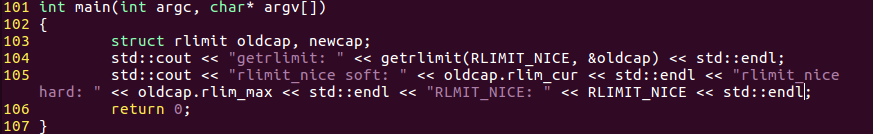
\includegraphics[width=0.9\textwidth]{../figures/systemgrundlagen/RLIMIT_NICE_code.png}}
	\subfigure[RLIMIT\_NICE output]{
		\label{RLIMIT_NICE_output}
		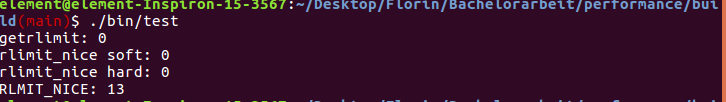
\includegraphics[width=0.9\textwidth]{../figures/systemgrundlagen/RLIMIT_NICE_output.png}}
	\caption{RLIMIT\_NICE} 
	\label{RLIMIT_NICE}
\end{figure*}
\\
Per default the process will have
the nice value of 0 and this value can be increased to the highest value allowed (-19), but cannot be
decreased afterwards to a value lower than \textit{user\_nice\_value = 20-RLIMIT\_NICE}. A way of
increasing the nice value would be to increase the RLIMIT\_NICE value (also as root or with root-rights = sudo), which will allow a normal user to increase the value given until it reaches
\dq user\_nice\_value\dq{}. Another way would be to log in as root, use the library's functions, build the program and set the SUID as root
\footnote{The SUID is a special bit that one can set and allows normal users to run the program as they
were root}.\\
At last you could also modify the \dq/etc/security/limits.conf\dq{} file and set a new max nice value for a
certain user, but this is not the best solution, because that user would have the power to change
priorities not only for one program, but for all its programs.
\subsubsection{Privileges}
As mentioned above, when a user wants to increase the priority of a thread or process, one has to either use special commands or be signed up as root. The reason for this is the way a processor works. There are commands that use the so called \textit{privileged} and \textit{unprivileged} instructions.\\
The privileged instructions can access every corner of a processor and has no memory restrictions, such as interrupt registers, control registers or registers that define on which frequency the CPU is running. The unprivileged instructions have restrictions to internal memory segments and attributes, such as changing the default scheduler or the capabilities of a process. This way, one can restrict some applications in order to not temper with critical system areas.\\
To simply explain this, let's take a look at the stack of a simpler CPU such as a cortex M4 and its registers pictured in figure \ref{cortex_M4_registers}\footnote{CPUs such as Intel or Ryzen are more complex, because they have to ensure the functionality of operating systems such as Windows or Linux, whereas Cortex processors are meant for embedded devices with simpler instruction set. However they also work with OS such as RTOS(real time operating systems)}.
\begin{figure}[!htbp]
	\centering
	\subfigure[Cortex M4 Stack]{\label{fig:a}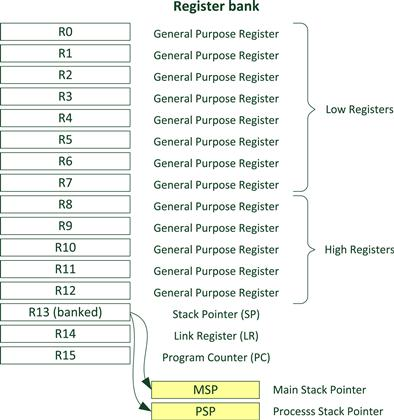
\includegraphics[scale=0.65]{../figures/systemgrundlagen/cortex_m4_stack.jpg}}
	\subfigure[Cortex M4 Special Regsiters]{\label{fig:b}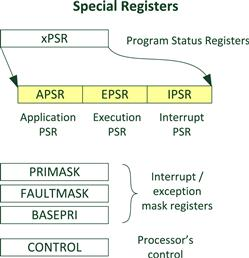
\includegraphics[scale=0.8]{../figures/systemgrundlagen/cortex_m4_special_registers.jpg}}
	\label{cortex_M4_registers}
\end{figure}
When a user writes a simple program such as the addition of some variables using the ALU\footnote{Arithmetic logical unit}, then this can be ran in unprivileged mode and so the processor will use only the registers in the \textit{Register Bank}. However if the user has a more complex program that uses for example interrupt routines from the peripheral of the CPU, which for example Intel processors constantly do for maintaining the system, then the code will have to use privileged code for setting the appropriate flags, which means the writing to registers such as the \textit{CONTROL} register, and then land in a ISR\footnote{Interrupt Service Routine}. Registers such as the CONTROL register can only be accessed by privileged instructions and are protected by the MPU\footnote{Memory protection unit}, because they have such power, that a wrong setting can shutdown the whole processor\cite{cortexM4}.
\subsubsection{Scheduling}
\label{ssec:sched_policies}
Unlike Windows, Linux has methods to change one's process and its threads scheduling policies.The default policy set on UNIX
is called "Round-Robin Timesharing" (SCHED\_OTHER). This allows jobs to be executed in a round robin fashion where
each process gets an equal time-slice of a CPU. There are more than one policy which can be set.
These are:
\begin{enumerate}
	\item SCHED\_OTHER
	\item SCHED\_BATCH
	\item SCHED\_IDLE
	\item SCHED\_FIFO(real time policy)
	\item SCHED\_RR(real time policy)
\end{enumerate}
The difference between SCHED\_RR (normal Round Robin scheduling) and "Round Robin Timeshare"(SCHED\_OTHER) is that the realtime policy lets
us to coordinate the priorities for that schedueling policy's queue.\\
SCHED\_BATCH and SCHED\_IDLE are two normal prioritised policies, which differ from SCHED\_OTHER, but
not enough for me to focus too much on them.
The only differences are that BATCH schedules a process less
frequently, if the it gets the CPU very often and IDLE is the equivalent to a process with a nice value of 19
(very nice process <=> lowest value).\\
You can get the current policy of your process by calling \texttt{int sched\_getscheduler(pid\_t pid)} from the \texttt{<sched.h>} header file. 
\\
Each of the policies mentioned above has a range of priorities levels, which can be get using the \texttt{sched\_get\_priority\_max(int policy)} and \texttt{sched\_get\_priority\_min(int policy)} methods found in \texttt{<sched.h>}\footnote{These can be different depending on the calling xUNIX
machine}.\\
On my Linux Notebook I have the following values shown in figure \ref{sched_prio_range}.
\begin{figure*}[!htb]
	\centering
	\subfigure[sched\_prio\_range code]{
		\label{sched_prio_range_code}
		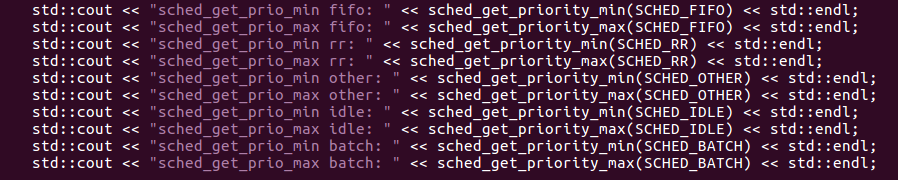
\includegraphics[width=0.9\textwidth]{../figures/sched_prio/sched_prio_range_source.png}}
	\subfigure[sched\_prio\_range output]{
		\label{sched_prio_range_output}
		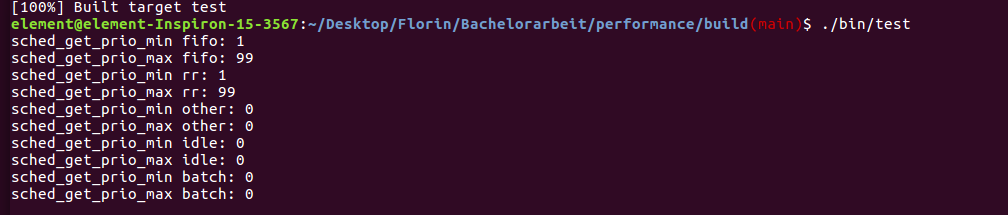
\includegraphics[width=0.9\textwidth]{../figures/sched_prio/sched_prio_range_output.png}}
	\caption{sched\_prio\_range} 
	\label{sched_prio_range}
\end{figure*}
\\
You can only change the priority of real-time policies, hence when you set the policy of a thread to OTHER, IDLE or BATCH you can't change the priority of that thread of execution.\\
As you can observe in figure \ref{sched_prio_range} only two of these have a \dq real\dq{} range.
SCHED\_RR and SCHED\_FIFO are characterized as real-time policies and have a higher priority than the
others. When two processes with SCHED\_RR and respectively SCHED\_FIFO have to share a CPU,
ironically the one that was placed first in that CPU's queue will get to run its job. Both of these
policies can lose access of their CPU, if they finish execution, call sched\_yield() or a syscall is called
and a higher priority process preempts them (a process with a lower nice value appears in the queue
or the user changes the value himself). SCHED\_RR can also lose its access if the timeslice if
the job expires.

\section{Synchronization}
When working with threads, the programmer cannot forget that these share the same stack, therefore they share the same variables. When two or more threads start their execution (eg. a simple addition), one cannot tell when will they perform what (if their priorities weren't tampered with).\\
There are two main operations threads can perform on a variable: \texttt{read()} and \texttt{write()}. Even a simple addition needs to first read the value from a register, add a number to it and then write the new value back to the register. Reading from a variable is not problematic, because its content will always stay the same, but writing to one is a whole different story. Let's take a look at the following code:
\begin{figure}[!htb]
	\centering
	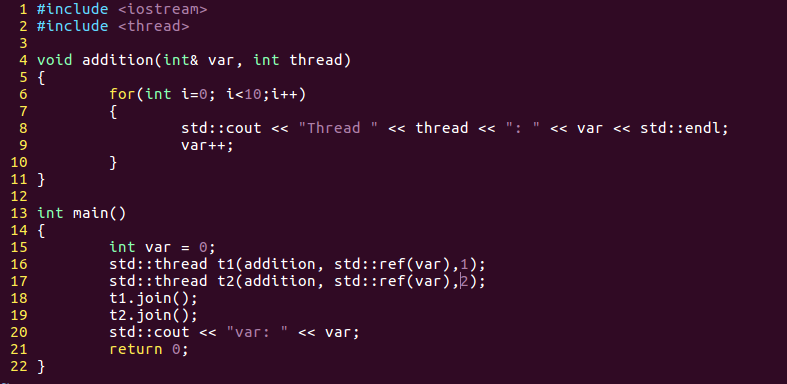
\includegraphics[width=0.5\textwidth]{../figures/systemgrundlagen/synchronizationExample.png}
	\caption{Thread's behavior without synchronization - Source code}
\end{figure}\\
\newpage
Here we create two threads with the sole purpose of adding a common variable. Most people would expect, because of the order of creation, for t1 to do his job and afterwards t2, but this is not the case.
\begin{wrapfigure}{1}{0.5\textwidth}
	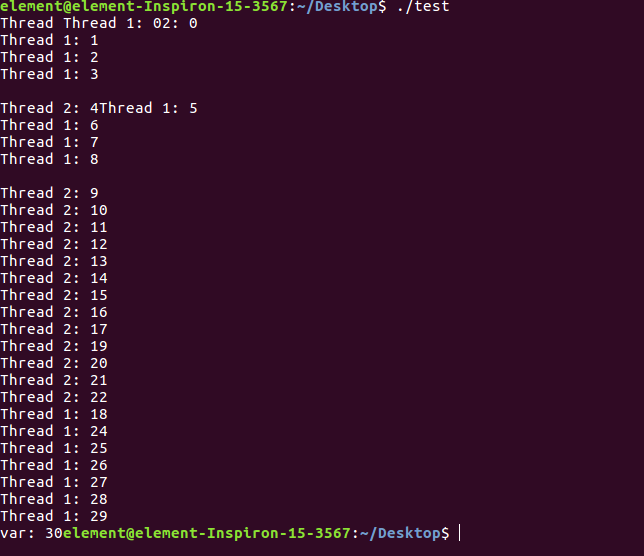
\includegraphics[width=.98\linewidth]{../figures/systemgrundlagen/synchronizationExampleOutput.png}
	\caption{Thread's behavior without synchronization - Output}
	\label{thread's_behavior}
\end{wrapfigure}

As you can observe in figure \ref{thread's_behavior}, the prints make no sense. The threads do not follow a sequentially pattern so the variable can be increased by \texttt{t1} for a time then by \texttt{t2} and for the rest of the remaining time by \texttt{t1} again.\\
Something that cannot be seen in the output would be the scenario when \texttt{t1} and \texttt{t2} try to access the variable and increment it at the same time. No one can accurately predict what the result would be (this is also known as \textit{ Unexpected behavior}). To resolve this problem in classic C people came up with the idea of a locking mechanism called \texttt{Mutex}.\\
\subsection{Mutex}
Mutexes are guards that can block other threads the access to variables inside a user-defined block of code (also known as \textit{scope}). These allow the thread that called \texttt{lock()} exclusive access to the variables inside that scope until the thread calls \texttt{unlock()}\cite{concurrency}. If another thread tries to lock the mutex for himself while the mutex is being used, then it will land in a waiting state until that lock is released.  The accessing order of the variable is \dq First come, first served\dq{}.\\
But as many implementations, this method can create problems, especially if the programmer forgets to \texttt{unlock()} the mutex. If this ever happens, it can lead to other threads being stucked in a waiting state forever (this is also called a \textit{Deadlock})\cite{cppExpert}.\\
This method requires a lot of concentration from the programmer and a good overview of all locking and release point.
Fortunately the \textit{Standard C++ Library} implemented new ways to use mutexes like \textit{lock\_guards}, which unlock themselves when the user goes out of scope, \textit{unique\_locks}, \textit{shared\_locks} and even \textit{timed\_mutexes}. Additionally they made a more simplistic technology for threads to access only common variable (and not a whole scope) called \textit{Atomic Variables}.
\subsection{Atomic Variables}
Atomic variables can be seen as wrappers for primitive data types, like \texttt{bool}, \texttt{int}, \texttt{double}, \texttt{float}, etc., but also for defined structs like \texttt{uint32\_t}, \texttt{uintptr\_t} or \texttt{int\_fast32\_t}\\
Basic syntax of this wrapper is: \textit{atomic<data\_type/class>} or (if defined) \textit{atomic\_data\_type} and it will grant the calling thread exclusive access to a certain variable while reading from or writing to it.\\
To read from an atomic variable one could just use the \dq =\dq{}-operator or (preferred) the \texttt{atomic\_var.load()} method. Writing to an atomic variable should only be done by using the \texttt{atomic\_var.store()} method, because this way you can expect that no one else besides the calling thread is accessing that variable\cite{stdAtomic, atomicConference}.\\
One must be very careful when using atomic operations on a variable.
To explain this in detail let's observe the following example:
\begin{center}
	A simple incrementation of a variable:
	\begin{enumerate}
		\centering
		\item x++
		\item x += 1
		\item x = x+1
	\end{enumerate}
\end{center}
All of these are atomic operation, but number three is different from the first two. The first and second operation are both \textit{atomic increments}. The third however, needs to apply more operations on the variable. Here there is an \textit{atomic read}, to get the value from x and store it in a register, afterwards we add one to it and there is an \textit{atomic write}, to set the variable to its new value. If you are working with multiple threads any other thread can come in between the \texttt{write} and the \texttt{read} and temper with the value, because there is no exclusivity while the value is stored in the register. 
The atomic library comes with additional member functions to make sequences of reading and writing easier and specialized member function that define bitwise operations on a variable, but they go way too deep in complexity and understanding for me to focus too much on them\cite{atomicConference}.
\section{CMake}
Despite the numerous implementations for the C++ language, there are still some hardships that need to be overcome when working with it. When it came to building, many people used os-dependent technologies such as the \textit{GNU Compile Collection}(short GCC) for Linux\cite{gcc} or MingW, which supports the usage of the GCC compiler, on Windows\cite{mingw}. Despite the existing methods, developing for multiple architectures was always complicated as code needed to be moved from one computer to the other and recompile, only to see that some incompatibilities still existed between the code's lines, because of small differences between compilers. The demand \dq for a cross-platform build environment\dq{} was so high, that a new tool called \textit{CMake} emerged.\\
\dq CMake is an extensible open-source system that manages the build process in an operating system and in compiler-independent manner\dq{}. As mentioned on their website, the system is used with native build environments and can be used to build binaries of a specific projects. These binaries can be executable files or compiled libraries such as \text{*.o}-files (also known as Object-files) on Linux or \textit{*.dll} (Dynamical Linked Library) on Windows. In order to use this program one has to first write basic text files and call them \textit{CMakeLists.txt}. The content of these files needs to be written in an interpreted language. Its Syntax goes as follows: \texttt{COMMAND(args...)}. Each subdirectory of the project needs to contain a \textit{CMakeLists.txt} file that will later be linked through a command to the main \textit{CMakeLists.txt} file\cite{cmake-overview}. 

\section{Need for action}
Although the presented technology uses the C and C++ syntax and logic, there is still no universal tool to cover the most relevant operating systems out there when it comes to the machine's performance. This is where this library comes in handy.\\
The goals are:
\begin{enumerate}
	\item summarize the complexity between operating systems into easy-to-understand methods
	\item supply the user with numerous operations to ensure homogeneity and flexibility usage in order to cover most user-cases in the industry 
	\item  encourage creative test-solving ways   
\end{enumerate}
% Nachfragen :S es sieht nicht ganz richtig aus 
%warum ge0stae ich die Library so wie sie ist?